\Transcb{yellow}{blue}{Time systems}
\begin{center}
{\red Solar Time}
\end{center}
%
\begin{itemize}
\item {\blue Elapsed time between two identical observed positions of the Sun}
\item[] Basis of our usual 24 hour day/night system
\item Definition : 1 day = 24 hours $\quad$ 1 hour = 60 min. $\quad$ 1 minute = 60 sec.
\item[] Time definition : 12:00h when the Sun is at the observer's meridian
\item Different locations have different values of the {\blue Local Time (LT)}
\item[] Definition : {\blue Greenwich is defined as origin at the $0^{\circ}$ meridian}
\item[$\ast$] Time rate varies (eccentricity of Earth's orbit and tilt of Earth's spin axis)
\item Use the mean rate which averages out these effects $\rightarrow$ {\blue Mean Solar Time}
\item So at each location we have two times
\begin{itemize}
\item Steady clock with noons 24 hours apart $\rightarrow$ {\blue Local Mean Time (LMT)}
\item Actual position of the Sun $\rightarrow$ {\blue Local Apparent Time (LAT)}
\end{itemize}
\item The difference between LAT and LMT is called the {\blue Equation of Time}
\item[$\ast$] The reference is the \colorbox{yellow}{Greenwich Time (GMT or GAT)} 
\end{itemize}

\Tr
\begin{center}
{\red Sidereal Time}
\end{center}
%
\begin{itemize}
\item {\blue Elapsed time between two identical observed positions of the same Star}
\item[] Closely related to Solar Time but not identical
\item Observer outside the Solar system :
\item[] The Earth spins around its axis in 1 "day"
\item[] The Earth rotates around the Sun in $n$ "days"
\item[] After 1 Solar orbit the Earth has made 1 extra revolution around its spin axis
\item[] $\rightarrow$ 1 sidereal day = $(1-1/n)$ solar day
\item Consequently : {\blue 1 sidereal day = 23h 56m 04.09s (Mean Solar Time)}
\item[] Time definition : Related to the coord. of a Star at the observer's meridian
\begin{itemize}
\item These coordinates will be explained later
\item These coord. vary due to precession and nutation of the Earth's spin axis
\end{itemize}
\end{itemize}

\Tr
\onecolumn
\begin{center}
{\blue Sidereal time versus Solar time}\\[3mm]
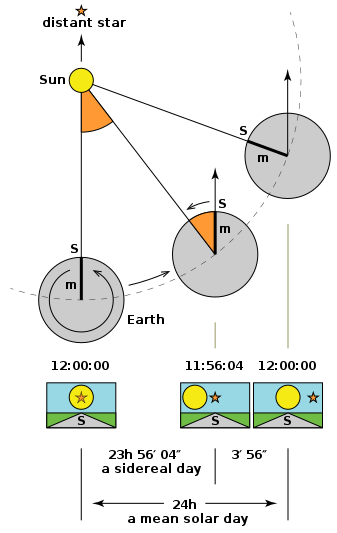
\includegraphics[keepaspectratio,height=14cm]{siderial-time}
\end{center}

\Tr
\begin{itemize}
\item Precession effect is stable and well known, nutation effect is more complex
\item[] Precession period : 25770 years
\item Use average epoch (50 years) coordinates to correct for the precession effect
\item[] $\rightarrow$ {\blue Mean Sidereal Time}
\item So at each location we have two times
\begin{itemize}
\item {\blue Local Mean Sidereal Time (LMST)} (i.e. precession included, nutation not)
\item {\blue Local Apparent Sidereal Time (LAST)} (incl. both precession and nutation)
\end{itemize}
\item[$\ast$] The reference is the \colorbox{yellow}{Greenwich Sidereal Time (GMST or GAST)} 
\item This looks all fine, but what determines the value of the time intervals ?
\item[] In other words : {\blue What counts the elapsed number of seconds ?}
\end{itemize}

\Tr
\begin{center}
{\red International Atomic Time (TAI)}
\end{center}
%
\begin{itemize}
\item The absolute value of the second is defined by atomic transitions
\item[] Remember that we used \Nuc{12}{6}{C} to define the atomic mass unit (amu)
\item \Nuc{133}{55}{Cs} has a hyperfine $4 \rightarrow 3$ transition of the $^{2}S$ ground state
\item[] This transition happens very frequently and at a very stable rate
\item[] {\blue 1 atomic (SI) sec. $\equiv$ 9192631770 cycles of this \Nuc{133}{55}{Cs} transition}
\item An individual Cs clock has a stability of the order of $10^{-14}$ per day
\item[] Using a set of Cs clocks all over the world provides even better stability 
\item[$\ast$] Basis of {\blue TAI : Temps Atomique International}
\item TAI : Stable time system but not linked with astronomical phenomena
\item[] TAI was introduced (= start epoch) 01-jan-1958 00:00:00 GAT
\item[] $\rightarrow$ \colorbox{yellow}{The reference for the absolute TAI time is Greenwich}
\item[] Earth's spin is irregular $\rightarrow$ Alternative for TAI needed
\end{itemize}

\Tr
\begin{center}
{\red Coordinated Universal Time (UTC)}
\end{center}
%
\begin{itemize}
\item Astronomical time standard : {\blue UTC (Temps Universel Coordonn\'{e})}
\item[] UTC transpires at the same rate as TAI $\rightarrow$ Clock ticks every SI second
\item[] Average correction for the irregular Earth spin by introducing {\blue leap seconds}
\item[$\ast$] The leap second correction was introduced on 01-jan-1972 00:00:00 GAT
\item[] This empirical correction is needed only every few years
\item[] See {\tt http://maia.usno.navy.mil/ser7/tai-utc.dat} for an overview
\item This implies : {\blue TAI-UTC=$\Delta$AT} $\quad$ Currently (2019) $\Delta$AT=37 sec. 
\item[$\ast$] UTC is broadcast via various servers using a Network Time Protocol (NTP)
\item[] See for instance {\tt http://www.time.gov} or {\tt http://www.time.gov/widget.html}
\item[$\ast$] \colorbox{yellow}{The reference for the absolute UTC time is Greenwich}
\item[] UTC is not updated for Daylight Saving Time (DST)
\item GPS timing was started at 06-jan-1980 00:00:00 UTC with $\Delta$AT=19 sec.
\item[] GPS clocks tick at the same rate as TAI $\rightarrow$ {\blue GPS=TAI-19 sec.} (fixed)
\end{itemize}

\Tr
\begin{center}
{\red Universal Time (UT1)}
\end{center}
%
\begin{itemize}
\item Time corrected for the actual Earth spin is called {\blue Universal Time (UT1)} 
\item[] This implies : {\blue UT1-UTC=$\Delta$UT1}
\item[] See {\tt https://hpiers.obspm.fr/iers/series/opa/eopc04} for daily updates
\item[$\ast$] $|\Delta$UT1$|$ is kept $<0.9$ sec. by introduction of leap seconds in UTC
\end{itemize}
%
\begin{itemize}
\item[] \begin{center}{\red Terrestrial Time (TT)}\end{center}
\item This is the TAI time corrected for GR effects at average sea level
\item[] Started at 01-jan-1977 00:00:00 TAI with {\blue TT $\equiv$ TAI+32.184 sec.}
\item[] This makes TT a continuation of the predecessor Ephemeris Time (ET)
\end{itemize}
%
\begin{itemize}
\item[] \begin{center}{\red Geocentric Coordinate Time (TCG)}\end{center}
\item The same as TT but for a reference frame not in the Earth's grav. potential
\item[] Relation : {\blue TCG $\approx$ TT+$7 \cdot 10^{-10} \Delta$T}
\item[] $\Delta T \equiv$ elapsed time in SI sec. since 01-jan-1997 00:00:00 TT
\end{itemize}

\Tr
\begin{center}
{\red Julian Date (JD)}
\end{center}
%
\begin{itemize}
\item Comparison of observations over many years is quite cumbersome
\begin{itemize}
\item Varying number of days in a year (leap years) and in various months
\item The absolute time indication is position dependent
\item Some sort of correction may have been applied at some time
\end{itemize}
\item Can't we have a steady ticking clock yielding an overall absolute reference ?
\item[] Yes we can !
\item A {\blue continuous day counting system} has been introduced called {\blue Julian Dates}
\item[] {\blue Origin JD=0} has been defined as {\blue 01-jan-4713 BC at 12:00:00 Greenwich}
\item[] Each {\blue Julian day} has exactly {\blue 86400 seconds}
\item[] No leap seconds are introduced
\item[] Each {\blue Julian century} has {\blue 36525 days} $\rightarrow$ Each {\blue Julian year} has {\blue 365.25 days}
\item Example : 02-jan-2000 12:00:00 UT corresponds to JD=2451546.0
\item[$\ast$] This day counting system can be used with any time system at Greenwich
\end{itemize}

\Tr
\begin{center}
{\red Modified Julian Date (MJD)}
\end{center}
%
\begin{itemize}
\item To avoid too large numbers a {\blue Modified Julian Date} has been introduced 
\item[] Same definitions as for the Julian Date but different origin
\item[$\ast$] {\blue Origin MJD=0} has been defined as {\blue 17-nov-1858 at 00:00:00 Greenwich}
\item[] Consequently : {\blue MJD=JD-2400000.5}
\item In practice MJD is used for calculations (computer accuracy), plots etc.
\end{itemize}
%
\begin{center}
{\red Julian Epoch (JE)}
\end{center}
%
\begin{itemize}
\item JE = fractional elapsed Julian year count since 01-jan-0000 12:00:00
\item[] Example : 01-jan-1965 12:00:00 UT corresponds to JE=1965.0
\end{itemize}
%
\begin{center}
{\red Besselian Epoch (BE)}
\end{center}
%
\begin{itemize}
\item BE = fractional elapsed Besselian year count since 01-jan-0000 12:00:00
\item[] A Besselian (tropical) year is defined to be 365.242198781 days
\end{itemize}
